\begin{activity} \label{A:10.6.12} 
  Figure \ref{F:10.6.gradient.field} shows a plot of the gradient
  $\nabla f$ at several points for some function $f(x,y)$.

  \begin{figure}[ht]
    \begin{center}
      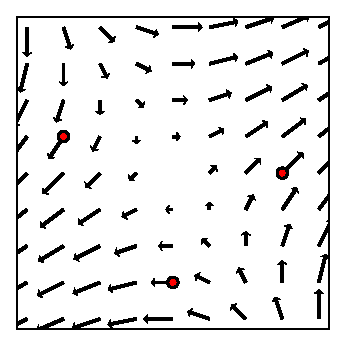
\includegraphics{figures/fig_10_6_gradient_field.eps}
    \end{center}	
    \caption{The gradient $\nabla f$.}
    \label{F:10.6.gradient.field}
  \end{figure}

  \ba
\item Consider each of the three indicated points, and draw, as best
  as you can, the contour line through that point.

\item Beginning at each point, draw a curve on which $f$ is continually
  decreasing. 

  \ea

\end{activity}
\aftera
